\section{Diagnostica supplementare dei trasferimenti e della formulazione ALE}
\label{app:transfer}

\subsection{Errore e costo dei trasferimenti}

Il benchmark dedicato agli operatori di trasferimento utilizza dieci target geometrici, mesh con 1089 nodi e 2048 triangoli e dieci ripetizioni temporali per misura. Le mediane riportate sono:
\begin{center}
\small
\begin{tabularx}{\columnwidth}{Xrr}
\toprule
Metrica & $P_1$ & $L^2$\\
\midrule
Errore relativo $L^2$ & 5.779\% & 3.811\%\\
Discrepanza relativa di massa & $5.892\times10^{-3}$ & $8.118\times10^{-5}$\\
Tempo mediano per trasferimento & 1.073 ms & 13.320 ms\\
\bottomrule
\end{tabularx}
\end{center}
La proiezione $L^2$ riduce l'errore e la discrepanza di massa nel campione diagnostico, ma costa circa 12.4 volte il trasferimento $P_1$. La discrepanza di massa qui riportata è quella definita nel benchmark di trasferimento; non viene equiparata a un residuo del bilancio PDE.

\subsection{Convergenza, qualità della mesh e tracking}

\begin{figure}[!htbp]
\centering
\IfFileExists{images/stage_a/stage_a_element_quality.pdf}{%
  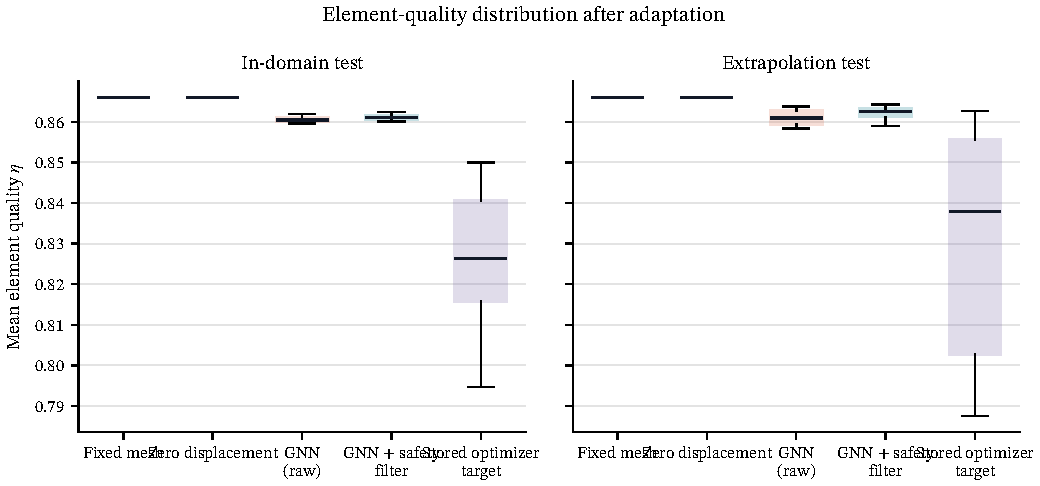
\includegraphics[width=0.95\columnwidth,height=0.28\textheight,keepaspectratio]{images/stage_a/stage_a_element_quality.pdf}%
}{%
  \fbox{\begin{minipage}[c][0.105\textheight][c]{0.88\columnwidth}
  \centering\footnotesize\textbf{Figura non inclusa nel pacchetto sorgente}\par\vspace{0.35em}
  \scriptsize\nolinkurl{images/stage_a/stage_a_element_quality.pdf}
  \end{minipage}}%
}
\caption{Qualità degli elementi nel benchmark statico Stage A.}
\label{fig:app_stagea_element}
\end{figure}
\begin{figure}[!htbp]
\centering
\IfFileExists{images/stage_a/stage_a_runtime_comparison.pdf}{%
  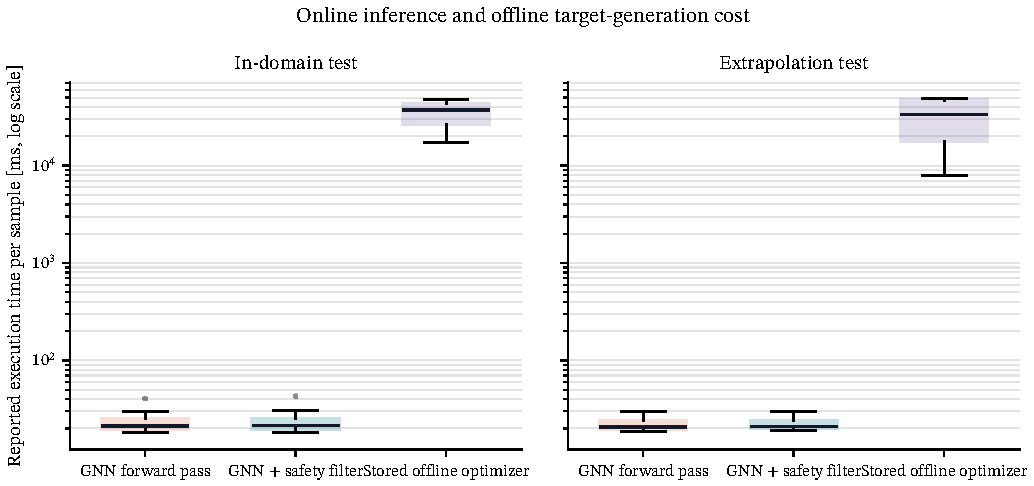
\includegraphics[width=0.95\columnwidth,height=0.28\textheight,keepaspectratio]{images/stage_a/stage_a_runtime_comparison.pdf}%
}{%
  \fbox{\begin{minipage}[c][0.105\textheight][c]{0.88\columnwidth}
  \centering\footnotesize\textbf{Figura non inclusa nel pacchetto sorgente}\par\vspace{0.35em}
  \scriptsize\nolinkurl{images/stage_a/stage_a_runtime_comparison.pdf}
  \end{minipage}}%
}
\caption{Tempo di inferenza e costo della pipeline statica Stage A.}
\label{fig:app_stagea_runtime}
\end{figure}
\begin{figure}[!htbp]
\centering
\IfFileExists{images/stage_a/fig3_safety_curve.pdf}{%
  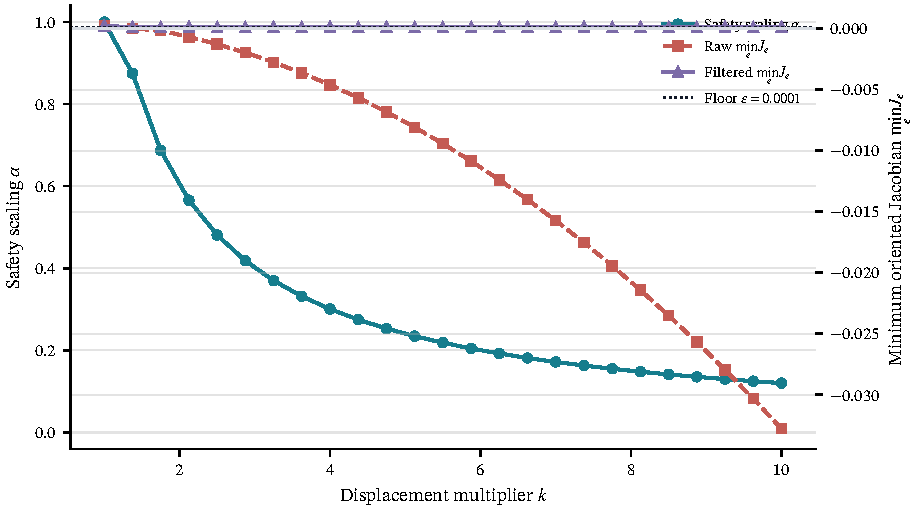
\includegraphics[width=0.95\columnwidth,height=0.28\textheight,keepaspectratio]{images/stage_a/fig3_safety_curve.pdf}%
}{%
  \fbox{\begin{minipage}[c][0.105\textheight][c]{0.88\columnwidth}
  \centering\footnotesize\textbf{Figura non inclusa nel pacchetto sorgente}\par\vspace{0.35em}
  \scriptsize\nolinkurl{images/stage_a/fig3_safety_curve.pdf}
  \end{minipage}}%
}
\caption{Curva di sicurezza geometrica del filtro nel benchmark Stage A.}
\label{fig:app_stagea_safety}
\end{figure}
\begin{figure*}[!t]
\centering
\IfFileExists{images/stage_a/fig4_runtime_scaling.pdf}{%
  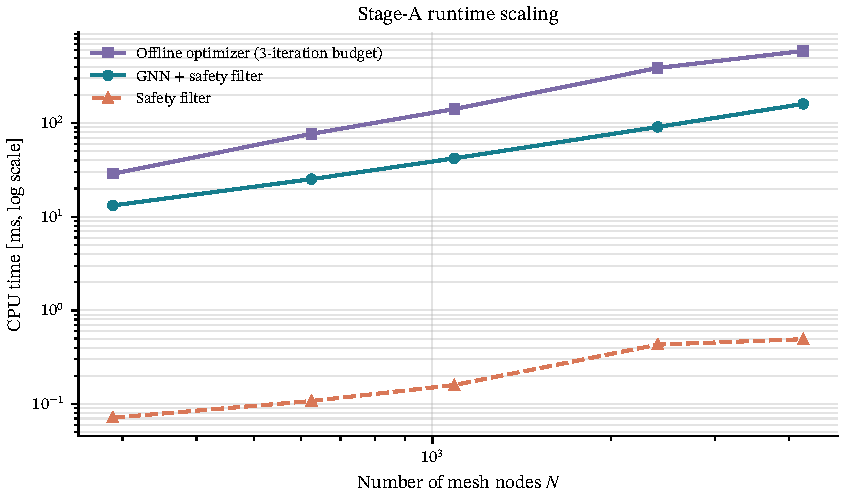
\includegraphics[width=0.95\textwidth,height=0.32\textheight,keepaspectratio]{images/stage_a/fig4_runtime_scaling.pdf}%
}{%
  \fbox{\begin{minipage}[c][0.105\textheight][c]{0.88\textwidth}
  \centering\footnotesize\textbf{Figura non inclusa nel pacchetto sorgente}\par\vspace{0.35em}
  \scriptsize\nolinkurl{images/stage_a/fig4_runtime_scaling.pdf}
  \end{minipage}}%
}
\caption{Andamento del costo di inferenza al variare della dimensione del grafo nel test Stage A.}
\label{fig:app_stagea_scaling}
\end{figure*}

La campagna Stage C ha inoltre verificato la risposta della discretizzazione ALE a differenti configurazioni di movimento, la qualità geometrica lungo la traiettoria e il costo dei componenti. I relativi risultati principali sono già sintetizzati nella Sezione~\ref{sec:stageabc}; in questa appendice si conservano le figure complementari per documentare le diagnostiche che non sono centrali nella narrazione dei risultati PDE Stage D.
